\documentclass[11pt]{article}
\usepackage{neurips_2026}

% Typography
\usepackage[protrusion=true,expansion=false,tracking=false]{microtype}

% Math
\usepackage{amsmath,amssymb,amsthm}
\usepackage{mathtools}
\usepackage{bm}

% Layout & figures
\usepackage{graphicx}
\usepackage{booktabs}
\usepackage{multirow}
\usepackage{enumitem}
\usepackage{wrapfig}
\usepackage{algorithm,algorithmic}
\usepackage[dvipsnames,svgnames,table]{xcolor}
\usepackage{colortbl}
\usepackage[utf8]{inputenc}
\usepackage[T1]{fontenc}
\usepackage[font=small,labelfont=bf,labelsep=period]{caption}

% Hyperlinks & cross-references
\usepackage[hidelinks,
  pdfauthor={Anonymous},
  pdftitle={Phantom Phases: How Attention Sinks Generate Fictitious Training Dynamics},
  bookmarksnumbered=true]{hyperref}
\usepackage[capitalize,noabbrev]{cleveref}

% Table spacing
\renewcommand{\arraystretch}{1.05}

% Float spacing compression
\setlength{\textfloatsep}{8pt plus 2pt minus 2pt}
\setlength{\floatsep}{8pt plus 2pt minus 2pt}
\setlength{\intextsep}{6pt plus 2pt minus 2pt}
\setlength{\abovecaptionskip}{4pt}
\setlength{\belowcaptionskip}{0pt}

% Colors (Okabe-Ito, colorblind-safe)
\definecolor{colRaw}{HTML}{D55E00}
\definecolor{colDS}{HTML}{0072B2}
\definecolor{colTheory}{HTML}{4477AA}
\definecolor{colPhase1}{HTML}{009E73}

\newtheorem{theorem}{Theorem}
\newtheorem{corollary}{Corollary}
\newtheorem{definition}{Definition}

\title{Phantom Phases: How Attention Sinks Generate\\Fictitious Training Dynamics}

\author{Anonymous Author(s)}

\date{}

\begin{document}
\maketitle

%======================================================================
\begin{abstract}
Standard spectral analysis of transformer training has revealed a rich narrative of geometric phases, rank collapse, and representational reorganization.
We offer an alternative explanation: these phenomena are generated by a single confound---the attention sink---that progressively dominates the very metrics used to observe it.
A one-parameter model of sink contamination predicts the observed $E_1$ trajectory with $R^2 = 0.978$, and removing the sink direction (\emph{de-sinking}) eliminates all apparent phase transitions.
Injecting a synthetic sink into clean representations reproduces the phantom trajectory from scratch, establishing a complete causal loop.
The true training dynamics tell a fundamentally different story: effective rank \emph{grows} ($191 \to 236$), not collapses ($178 \to 6.4$); raw effective rank is significantly \emph{anti-correlated} with model capability across models ($\rho = -0.59$ to $-0.72$, $p < 0.02$); and inter-layer CKA drops by up to 0.57, revealing layer differentiation hidden beneath a shared artifact.
Moreover, de-sinking uncovers a previously invisible phenomenon: hidden-state alignment with the unembedding matrix peaks early in training then declines---a \emph{shortcut-to-full-rank transition} observed across Pythia (70M--410M, all peaking at step 512) and OLMo-2 1B (step 1{,}000).
We quantify contamination across five metrics, models from 70M to 6.9B parameters, and both GPT-NeoX and GQA architectures, finding distortions up to $721\times$.
\end{abstract}

%======================================================================
\section{Introduction}\label{sec:intro}

\citet{li2025tracing} recently identified three non-monotonic geometric phases in transformer pretraining: an initial representational collapse, a period of dimensionality expansion, and a final compression phase correlated with downstream capability.
Their finding, published at NeurIPS~2025, synthesized a growing body of evidence from five independent spectral metrics---PCA variance concentration ($E_1$), effective rank, RankMe, CKA, and anisotropy---each independently suggesting that transformer training proceeds through abrupt geometric reorganizations~\citep{garrido2023rankme,ethayarajh2019contextual,raghu2021vision,timkey2021all}.
The convergence of multiple metrics on the same narrative has been taken as strong evidence that these phases are real properties of training dynamics.

We show that this convergence has a simpler explanation.
All five metrics share a single blind spot: the \emph{attention sink}~\citep{xiao2024efficient}, an input-invariant, high-norm component at position~0 whose magnitude grows monotonically during training.
Because this one component dominates the principal spectrum, any metric sensitive to variance concentration will track \emph{sink growth} rather than representational change---producing coherent but fictitious structure.
The apparent convergence across metrics is not independent confirmation; it is five measurements of the same artifact.

This claim is testable.
If geometric phases are driven by sink contamination rather than representation dynamics, then (1)~a contamination model with sink strength as the sole variable should predict the observed $E_1$ trajectory; (2)~removing the sink direction should eliminate all phase transitions; and (3)~the decontaminated metrics should tell a qualitatively different story.
All three predictions hold.
A single-parameter model fits $E_1$ with $R^2 = 0.978$ (Theorem~\ref{thm:e1}).
De-sinking eliminates Phases~2--3 entirely.
And the decontaminated effective rank shows monotonic \emph{growth} ($191 \to 236$), the opposite of the collapse ($178 \to 6.4$) reported by raw metrics.
Moreover, injecting a synthetic sink into clean representations reproduces the entire phantom trajectory from scratch (\S\ref{sec:manufacture}), completing the causal loop: the attention sink is both necessary and sufficient to produce the observed spectral artifacts.
Raw effective rank is not merely noisy but \emph{actively misleading}: it is significantly anti-correlated with probing accuracy across models ($\rho = -0.59$ to $-0.72$, $p < 0.02$), suggesting the model is deteriorating at exactly the steps where it is learning most rapidly.

De-sinking does more than correct existing measurements---it reveals new ones.
With the dominant artifact removed, we observe a previously invisible training phenomenon: hidden-state alignment with the unembedding matrix peaks early in training then declines.
This \emph{shortcut-to-full-rank transition} occurs at step~512 across all three Pythia model sizes (70M/160M/410M) and at step~1{,}000 in OLMo-2 1B, suggesting an intrinsic property of transformer optimization: models first learn a low-rank shortcut (the marginal token distribution), then depart toward richer, full-rank representations.

\paragraph{Contributions.}
\begin{enumerate}[leftmargin=1.5em,itemsep=0pt,topsep=1pt]
    \item \textbf{Sink contamination} (\S\ref{sec:theory}--\ref{sec:scope}): five standard spectral metrics are systematically biased by the attention sink. Rogue dimensions $\approx$ sink direction (95.7\% overlap). The effect is specific to PC1. A single-parameter contamination model achieves $R^2 = 0.978$. Injecting a synthetic sink into clean representations reproduces the phantom trajectory, completing the causal loop.
    \item \textbf{Phantom phases dissolved} (\S\ref{sec:true}): de-sinking eliminates geometric phases and reverses rank collapse to rank growth across three model sizes (70M/160M/1.4B). Raw ER is significantly anti-correlated with capability ($\rho = -0.59$ to $-0.72$, $p < 0.02$).
    \item \textbf{A hidden training transition revealed} (\S\ref{sec:alignment}): unembedding alignment peaks then declines---universal across four model families, with a depth-dependent inverted-U departure profile.
    \item \textbf{Scale and architecture validated} (\S\ref{sec:scope}): contamination spans GPT-NeoX and GQA architectures (Qwen2.5: sink $\alpha$ up to $113\times$, spectral gap $154\times$) and worsens with model size, reaching $721\times$ ER distortion at 6.9B.
\end{enumerate}

%======================================================================
\section{Background and Related Work}\label{sec:related}

\paragraph{Attention sinks.}
\citet{xiao2024efficient} identified disproportionate attention to the first token; \citet{darcet2024vision} proposed register tokens for ViTs.
Sinks arise from the softmax constraint~\citep{sun2024massive}, emerge early and strengthen with scale~\citep{gu2025attention}, and serve computational roles with near-zero value states~\citep{barbero2025why}.
\citet{cancedda2024spectral} decomposed sink signals via the unembedding spectrum.
\citet{zhang2025catch} showed 1--2 sink ``tags'' explain 20--70\% of PCA variance in attention outputs.
\citet{queipodellano2025sinks} proved massive activations \emph{necessarily} collapse effective rank, interpreting this as functional compression.
Their Theorem~1 is \emph{static} (sinks collapse ER at a given layer); our Theorem~\ref{thm:e1} establishes the \emph{dynamic} consequence: phantom phase transitions across training checkpoints.
They study what sinks \emph{are}; we study what sinks \emph{do to training-dynamics measurements}.

\paragraph{Spectral training dynamics.}
\citet{li2025tracing} identified three geometric phases using RankMe/$\alpha$-ReQ on OLMo and Pythia.
$E_1$/anisotropy: \citet{ethayarajh2019contextual}; rogue dimensions: \citet{timkey2021all}; RankMe: \citet{garrido2023rankme}; CKA: \citet{kornblith2019similarity}.
\citet{kulkarni2026disentangling} trained 108 models and found effective rank primarily reflects hyperparameters (batch size, weight decay)---a \emph{different} confound from ours.
None of these works controls for the attention sink.

\paragraph{Unembedding alignment.}
The logit lens~\citep{nostalgebraist2020logit} and tuned lens~\citep{belrose2023eliciting} established that alignment varies across \emph{layers} in trained models.
No prior work tracks alignment across \emph{training time}.

\paragraph{Simplicity bias.}
\citet{chang2022word} showed models acquire words in frequency order; \citet{cagnetta2024distributional} demonstrated transformers learn interactions from low to high order.
These support interpreting our alignment peak as a shortcut phase.

%======================================================================
\section{The Attention Sink Contaminates Spectral Metrics}\label{sec:theory}

\subsection{De-Sinking}\label{sec:desink}

\begin{definition}[De-sinking]
Let $\mathbf{H} \in \mathbb{R}^{n \times d}$ be hidden states.
Let $\mathbf{s} \in \mathbb{R}^d$ be the first right singular vector of the centered $\mathbf{H}$.
The de-sinked representations are $\mathbf{H}_{\text{ds}} = \mathbf{H} - (\mathbf{H}\mathbf{s})\mathbf{s}^\top$.
\end{definition}

\begin{algorithm}[t]
\caption{De-sinking}\label{alg:desink}
\begin{algorithmic}[1]
\REQUIRE Hidden states $\mathbf{H} \in \mathbb{R}^{n \times d}$
\STATE $\bar{\mathbf{H}} \leftarrow \mathbf{H} - \frac{1}{n}\mathbf{1}\mathbf{1}^\top\mathbf{H}$ \COMMENT{Center}
\STATE $\mathbf{U}, \mathbf{\Sigma}, \mathbf{V}^\top \leftarrow \text{SVD}(\bar{\mathbf{H}})$ \COMMENT{Thin SVD}
\STATE $\mathbf{s} \leftarrow \mathbf{V}_{:,1}$ \COMMENT{Sink direction}
\STATE $\mathbf{H}_{\text{ds}} \leftarrow \mathbf{H} - (\mathbf{H}\mathbf{s})\mathbf{s}^\top$ \COMMENT{Project out}
\RETURN $\mathbf{H}_{\text{ds}}$
\end{algorithmic}
\end{algorithm}

Both this method and an alternative (normalized mean of position-0 across sequences) yield nearly identical directions (\S\ref{sec:controls}), confirming that PC1 in sink-affected layers \emph{is} the sink direction.

\paragraph{De-sinking is specific, not generic.}
De-sinking operationally resembles All-but-the-Top~\citep{mu2018allbutthetop} and its extensions~\citep{li2020bertflow,rajaee2021cluster}, but serves a different purpose: it is a \emph{diagnostic correction} for training dynamics analysis, grounded in Theorem~\ref{thm:e1}, not an engineering recipe for downstream performance.
The effect is specific to PC1: removing PC2, PC3, or a random direction produces negligible change (Appendix~\ref{app:specificity}).
The spectral gap between the first and second singular values provides a principled justification for removing exactly one direction: in GPT-2, the gap exceeds $14\times$ at L2--L4, while in Pythia-70M it reaches $4.6\times$ at L2.
Non-sink layers show gaps of $1$--$2\times$.

\subsection{Why Contamination Is Inevitable}\label{sec:theorem}

The attention sink creates a component that is (i)~high-variance, (ii)~input-invariant, and (iii)~shared across layers.
We show contamination follows from (i) alone.

\begin{theorem}[$E_1$ Contamination]\label{thm:e1}
Let $\mathbf{H} = \alpha\,\mathbf{a}\mathbf{s}^\top + \mathbf{C}$, where $\mathbf{s}$ is a unit vector, $\|\mathbf{a}\|^2/n = \sigma_s^2$, and $\mathbf{C}\mathbf{s} \approx \mathbf{0}$.
Let $\boldsymbol{\Sigma}_c = \frac{1}{n}\mathbf{C}^\top\mathbf{C}$ have trace $V_c$.
Then:
\begin{equation}\label{eq:e1}
    E_1^{\textup{raw}} = \frac{\kappa\,\alpha^2 + E_1^c}{\kappa\,\alpha^2 + 1}\,,
    \qquad \kappa = \sigma_s^2 / V_c\,.
\end{equation}
As $\alpha \to \infty$, $E_1^{\textup{raw}} \to 1$ regardless of $E_1^c$.
\end{theorem}

\begin{proof}[Proof sketch]
Under orthogonality, $\boldsymbol{\Sigma} = \alpha^2\sigma_s^2\,\mathbf{s}\mathbf{s}^\top + \boldsymbol{\Sigma}_c$.
Largest eigenvalue $\lambda_1 \approx \alpha^2\sigma_s^2$; total variance $\alpha^2\sigma_s^2 + V_c$.
Full proof in Appendix~\ref{app:proof}.
\end{proof}

\begin{corollary}[Effective Rank Collapse]
As $\alpha \to \infty$, $\mathrm{ER} \to 1$ regardless of $\mathrm{ER}(\mathbf{C})$.
\end{corollary}

\begin{corollary}[CKA Homogenization]
Layers sharing sink direction $\mathbf{s}$ have $\mathrm{CKA} \to 1$ as sink strength grows.
\end{corollary}

\begin{corollary}[Anisotropy Inflation]
Average pairwise cosine similarity increases with $\alpha$.
\end{corollary}

Theorem~\ref{thm:e1} is not merely diagnostic---it is \emph{predictive}.
Given any content matrix $\mathbf{C}$ and sink strength $\alpha$, it predicts the exact degree of contamination.
This means phantom phases can be manufactured from first principles: any training run where sink strength grows monotonically will produce apparent rank collapse in raw metrics, regardless of what the content representations actually do.

\subsection{Empirical Validation}\label{sec:validation}

We validate on Pythia-70M~\citep{biderman2023pythia}, 20 checkpoints (steps 0--143{,}000).
Sink strength grows from $1.06\times$ at step~32 to $10.3\times$ at step~64{,}000.

\begin{figure}[t]
\centering
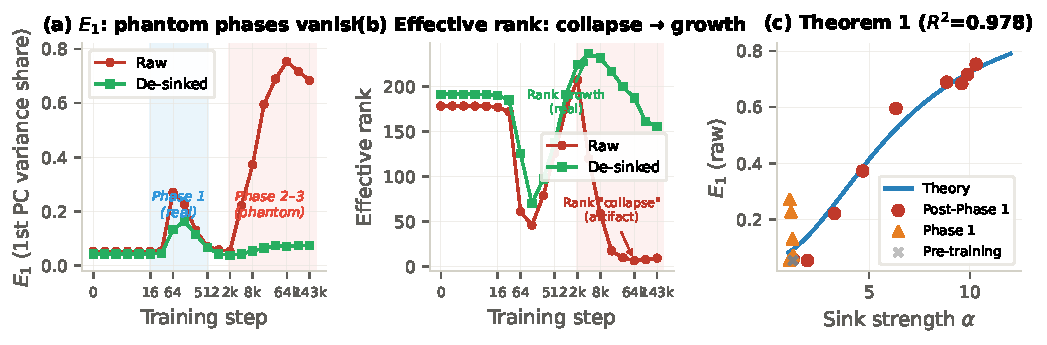
\includegraphics[width=\textwidth]{figs/fig1_hero.pdf}
\caption{\textbf{Phantom phases in transformer training (Pythia-70M, L3).}
\textbf{(a)}~Phases~2--3 vanish after de-sinking; only Phase~1 (blue) survives.
\textbf{(b)}~``Rank collapse'' ($178 \to 6.4$) reverses to rank \emph{growth} ($191 \to 236$).
\textbf{(c)}~Theorem~\ref{thm:e1} predicts contamination with $R^2 = 0.978$ (one parameter). Phase~1 points (triangles) deviate---content genuinely reorganizes during this period.}
\label{fig:hero}
\end{figure}

Figure~\ref{fig:hero}(c) shows the fit: $\kappa = 0.024$ yields $R^2 = 0.978$.
Phase~1 transient points (${\sim}$step 32--512) deviate from theory because content representations genuinely reorganize during this period---precisely the behavior expected if Phase~1 is a real training transition and Phases~2--3 are artifacts of sink growth.

\paragraph{Model robustness.}
Theorem~\ref{thm:e1} (1 param, $R^2 = 0.978$, AIC $= -127.8$) outperforms the best generic alternative (logistic, 3 params, $R^2 = 0.945$, AIC $= -105.3$) because it leverages content information via $E_1^c$.
Leave-3-out cross-validation (20 splits) yields $R^2 = 0.972$; Phase~1 residuals are $1.55\times$ larger than non-Phase-1, consistent with genuine representational change during that period.

\subsection{Manufacturing Phantom Phases}\label{sec:manufacture}

The evidence so far establishes \emph{necessity}: removing the sink eliminates phantom structure.
We now establish \emph{sufficiency}: injecting a synthetic sink into clean representations produces phantom structure from scratch.

Starting from Pythia-70M at step~512---where the sink has not yet formed ($\alpha \approx 1.0$)---we de-sink the hidden states, then add a rank-1 perturbation along the empirical sink direction with controlled strength $\alpha$.
As $\alpha$ grows from 0 to 30, $E_1$ rises from 0.063 to 0.898 and ER collapses from 140 to 2.3 (Appendix~\ref{app:manufacture})---reproducing the entire phantom trajectory from clean representations.
Combined with the removal experiments (\S\ref{sec:validation}), this completes a causal loop: the attention sink is both necessary \emph{and} sufficient to produce the observed spectral artifacts.

%======================================================================
\section{Scope of Contamination}\label{sec:scope}

\subsection{Five Metrics, Two Model Families}\label{sec:fivemetrics}

We apply de-sinking to GPT-2~\citep{radford2019language} (124M) and Pythia-70M on 200K tokens from OpenWebText.

\begin{table}[t]
\centering
\caption{\textbf{Contamination audit.} Maximum effect across layers.}
\label{tab:audit}
\small
\begin{tabular}{@{}llcccc@{}}
\toprule
\textbf{Metric} & \textbf{Reference} & \textbf{GPT-2 raw} & \textbf{GPT-2 ds} & \textbf{Pythia raw} & \textbf{Pythia ds} \\
\midrule
$E_1$ share & \citet{li2025tracing} & 93.6\% & 11.5\% & 62.6\% & 7.0\% \\
Rogue dims & \citet{timkey2021all} & 93.7\% & 14.6\% & --- & --- \\
\quad sink overlap & & \multicolumn{2}{c}{95.7\%} & --- & --- \\
RankMe & \citet{garrido2023rankme} & 352 & 612 & 355 & 415 \\
Anisotropy & \citet{ethayarajh2019contextual} & 0.55 & 0.48 & 0.98 & 0.13 \\
CKA (max $|\Delta|$) & \citet{raghu2021vision} & \multicolumn{2}{c}{$-0.569$} & \multicolumn{2}{c}{$+0.474$} \\
\bottomrule
\end{tabular}
\end{table}

The most striking result: the sink direction accounts for 90--96\% of rogue dimension variance at L3--L10 in GPT-2.
The ``rogue dimensions'' that \citet{timkey2021all} identified as obscuring representational quality \emph{are} the attention sink.
This single observation unifies two previously disconnected literatures.

\begin{figure}[t]
\centering
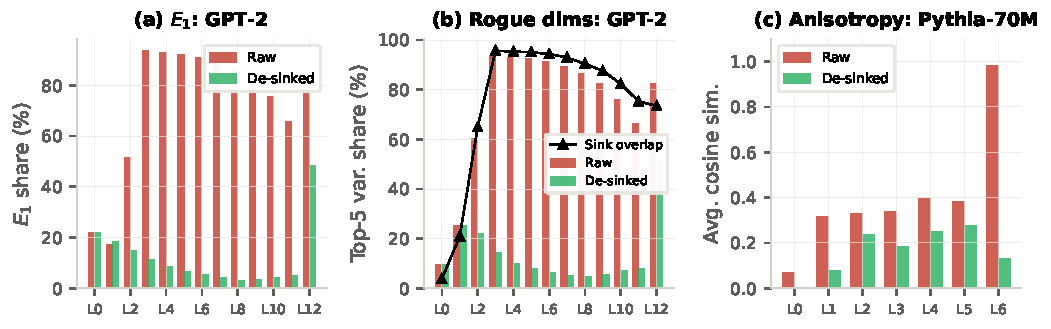
\includegraphics[width=\textwidth]{figs/fig2_metrics.pdf}
\caption{\textbf{Metric contamination across layers.}
\textbf{(a)}~$E_1$ in GPT-2: raw 94\%, de-sinked 3--12\%.
\textbf{(b)}~Rogue dimensions and sink overlap ($>$90\% at L3--L10).
\textbf{(c)}~Anisotropy in Pythia-70M: L6 drops from 0.98 to 0.13.}
\label{fig:metrics}
\end{figure}

\subsection{CKA Reveals Hidden Layer Differentiation}\label{sec:cka}

An aggregate CKA comparison suggests minimal impact (GPT-2: $0.703 \to 0.610$).
This masks the truth.

\begin{figure}[t]
\centering
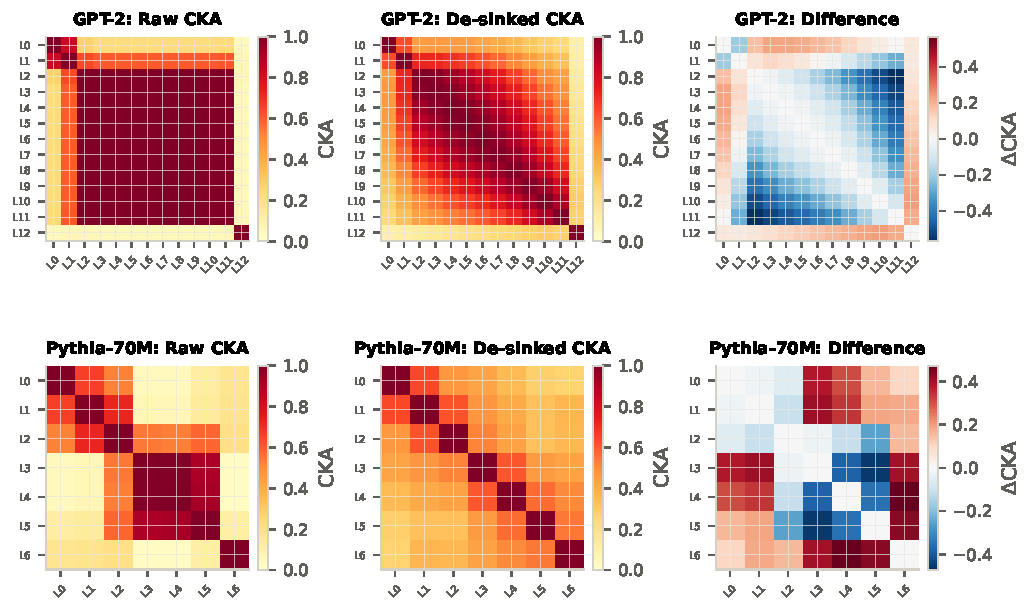
\includegraphics[width=\textwidth]{figs/fig3_cka.pdf}
\caption{\textbf{CKA heatmaps.} Top: GPT-2. Raw CKA shows L2--L11 as virtually identical ($\approx 1.0$); de-sinked CKA reveals a rich gradient structure (max $|\Delta| = 0.569$). Bottom: Pythia-70M.}
\label{fig:cka}
\end{figure}

Raw CKA shows L2--L11 as virtually identical ($\approx 1.0$), consistent with the narrative that deep layers ``converge'' during training.
De-sinked CKA reveals a monotone gradient from L2 to L11 (max $|\Delta| = 0.569$), consistent with progressive refinement---layers are \emph{differentiated}, not converged (Figure~\ref{fig:cka}).

\subsection{Contamination Worsens with Scale}\label{sec:scale}

\begin{table}[t]
\centering
\caption{\textbf{Contamination worsens with scale and spans architectures.} $^\dagger$Full 20-checkpoint training dynamics. $^\ddagger$GQA architecture (grouped-query attention, RoPE, SwiGLU).}
\label{tab:scale}
\small
\begin{tabular}{@{}lccccc@{}}
\toprule
\textbf{Model} & \textbf{Params} & \textbf{Max $E_1$ inflation} & \textbf{Max ER distortion} & \textbf{Peak $\alpha$} & \textbf{Peak layer} \\
\midrule
Pythia-70M$^\dagger$ & 70M & $16\times$ & $30\times$ & $10.3\times$ & L3 \\
GPT-2 & 124M & $17\times$ & $165\times$ & --- & L3 \\
Pythia-160M$^\dagger$ & 160M & $6.5\times$ & $6.9\times$ & $10.4\times$ & L5 \\
GPT-2-XL & 1.5B & $15\times$ & $290\times$ & --- & L12 \\
Pythia-1.4B$^\dagger$ & 1.4B & $6.6\times$ & $8.5\times$ & $14.8\times$ & L12 \\
\rowcolor{gray!8}
Qwen2.5-1.5B$^\ddagger$ & 1.5B & $29\times$ & --- & $113\times$ & L2 \\
Pythia-6.9B & 6.9B & $40\times$ & $721\times$ & --- & L8 \\
\bottomrule
\end{tabular}
\end{table}

\begin{figure}[t]
\centering
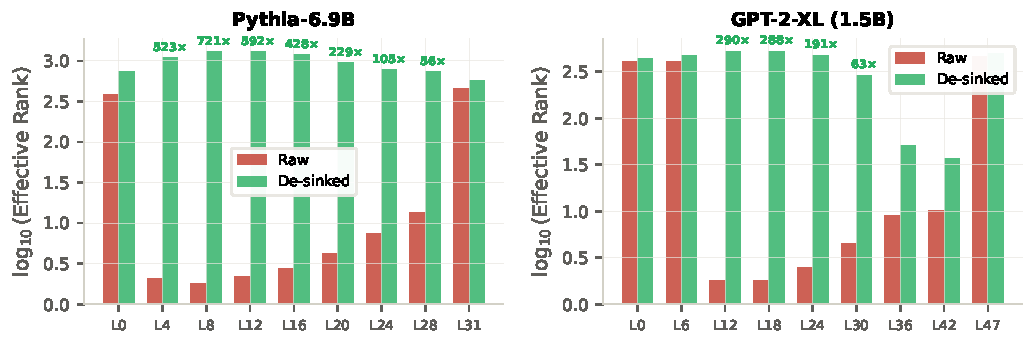
\includegraphics[width=\textwidth]{figs/fig4_scale.pdf}
\caption{\textbf{Contamination worsens with scale.} ER (log scale) for Pythia-6.9B and GPT-2-XL. Pythia-6.9B L8: $721\times$ distortion.}
\label{fig:scale}
\end{figure}

This trend has an uncomfortable implication: the larger the model, the less reliable standard spectral analysis becomes.
For Pythia-1.4B, sink strength reaches $14.8\times$ (vs.\ $10.3\times$ for 70M), and the raw ER collapse is more severe: $23 \to 2.7$ while de-sinked ER shows growth to $27.2$ before plateauing.
The pattern extends beyond the GPT-NeoX family: Qwen2.5-1.5B, which uses grouped-query attention (GQA), RoPE, and SwiGLU---the dominant modern architecture---exhibits \emph{even more extreme} contamination, with sink strength reaching $113\times$ and spectral gaps exceeding $150\times$ (Table~\ref{tab:scale}).
The phantom dynamics are not a small-model or old-architecture curiosity---they intensify at scale and generalize across architectures.

%======================================================================
\section{The True Training Dynamics}\label{sec:true}

\subsection{Rank Growth, Not Collapse}\label{sec:growth}

Figure~\ref{fig:hero}(b) shows the central positive finding.
After de-sinking, Pythia-70M L3 shows: stable ER~$\approx 190$ (steps 0--32); a genuine Phase~1 dip and recovery (steps 32--512); rank \emph{growth} from 138 to 236 (steps 512--8{,}000); and gradual plateau.
The ``rank collapse'' from 178 to 6.4 is entirely a sink artifact.

This pattern reproduces across scales.
Pythia-160M L5: raw ER collapses from 10.8 to 1.8 while de-sinked ER grows from 9.9 to 12.4.
Pythia-1.4B L12: raw ER collapses from 23.0 to 2.7 while de-sinked ER grows from 23.3 to 27.2 before plateauing at 17.9.
In all three models, de-sinking reverses the sign of the ER trajectory.

\subsection{Raw Metrics Give the Wrong Sign}\label{sec:misleading}

The contamination does not merely add noise---it reverses the direction of the signal.
Over 20 checkpoints, raw effective rank is significantly \emph{anti-correlated} with probing accuracy at sink-dominated layers: Pythia-70M L3 yields Spearman $\rho = -0.59$ ($p = 0.017$); Pythia-160M L3 yields $\rho = -0.72$ ($p = 0.002$).
De-sinked ER corrects this directional error (70M: $\rho = +0.25$; 160M: $\rho = -0.33$, n.s.), removing the significant misleading signal in both cases.

A researcher monitoring raw ER would conclude the model is deteriorating at exactly the steps where it is learning most rapidly.

\subsection{Only Phase~1 Survives}\label{sec:phase1}

Phase~1 (${\sim}$step 32--128) appears in \emph{both} raw and de-sinked metrics: de-sinked $E_1$ shows a transient spike ($0.04 \to 0.16 \to 0.04$), de-sinked ER drops and recovers, and perplexity plummets from $>10^6$ to 168.
Phases~2--3 exist only in raw metrics and track the growth of sink norm ratio.

Of the three geometric phases reported by \citet{li2025tracing}, one is real and two are phantom.

%======================================================================
\section{A Hidden Training Transition}\label{sec:alignment}

De-sinking does more than correct existing measurements---it clears the spectral foreground, making subtler geometric signals measurable.
We now show that one such signal reveals a previously invisible training phenomenon.

We define \emph{lm100 alignment} as the fraction of hidden-state variance captured by the top-100 singular vectors of $\mathbf{W}_{\text{lm\_head}}$.

\subsection{The Alignment Peak}\label{sec:peak}

\begin{figure}[t]
\centering
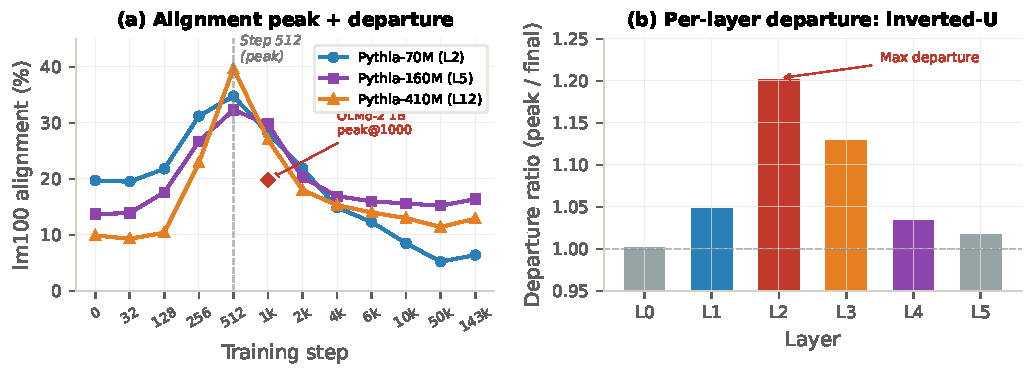
\includegraphics[width=\textwidth]{figs/fig5_alignment.pdf}
\caption{\textbf{The shortcut-to-full-rank transition.}
\textbf{(a)}~lm100 alignment peaks at step~512 across all Pythia sizes, then declines. OLMo-2 1B peaks at step~1{,}000 (diamond).
\textbf{(b)}~Per-layer departure ratio follows an inverted-U: middle layers depart most.}
\label{fig:alignment}
\end{figure}

Figure~\ref{fig:alignment}(a) shows the trajectory.
Early in training, alignment rises sharply as models learn the marginal token distribution---efficiently solved by aligning hidden states with the unembedding matrix's high-gain directions.
After step~512, alignment declines: the model transitions from this low-rank shortcut to full-rank encoding.

Four observations confirm this is genuine:
\textbf{(i)}~de-sinked ER expands rapidly at the alignment peak (Pythia-410M: $30 \to 49$ at steps 512--1{,}000);
\textbf{(ii)}~all Pythia models peak at step~512 despite different loss values---step-driven, not loss-driven;
\textbf{(iii)}~OLMo-2 1B (Llama architecture) peaks at step~1{,}000, confirming architecture-generality;
\textbf{(iv)}~sink $E_1$ is only 10.8--13.7\% at peak, so the alignment signal is independent of the sink.

\subsection{Middle Layers Depart Most}\label{sec:inverted}

The departure profile follows an inverted-U (Appendix~\ref{app:inverted}): L0 never aligns strongly (peak 29\%) and cannot depart; L5 is structurally constrained to remain aligned for prediction; middle layers (L2: $1.21\times$) depart most because they face alignment pressure from the gradient \emph{and} have downstream layers to compensate.

\subsection{Interpretation: From Shortcut to Full-Rank Computation}\label{sec:interpret}

Early training aligns hidden states with the unembedding matrix---a low-rank shortcut for the marginal token distribution~\citep{chang2022word,cagnetta2024distributional}.
As high-frequency tokens saturate, the model departs toward full-rank, context-dependent representations.
This transition is invisible in raw metrics because the attention sink dominates the principal spectrum during exactly this period.

%======================================================================
\section{Mechanism: Computationally Necessary, Informationally Empty}\label{sec:mechanism}

\paragraph{Causal necessity.}
Zeroing position-0 hidden states causes perplexity to explode $8\times$--$107{,}000\times$.

\paragraph{Informational emptiness.}
Linear probing shows $|\Delta| < 0.3\%$ at L0--L5.
At the final layer, de-sinking \emph{improves} probing by $+12.1\%$ (Pythia-70M) and $+8.3\%$ (Pythia-160M)---the sink interferes with readout when aligned with the unembedding matrix (cosine $0.97$--$0.99$ in Pythia; $0.26$ in GPT-2).

\begin{wrapfigure}[14]{r}{0.36\textwidth}
    \vspace{-1.2em}
    \centering
    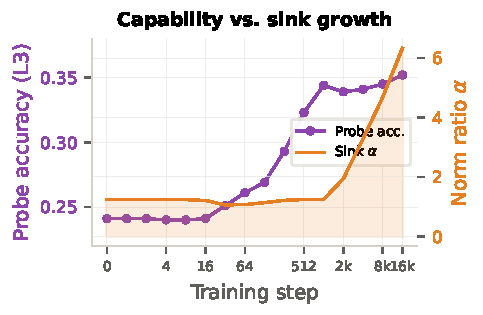
\includegraphics[width=0.36\textwidth]{figs/fig6_timeline.pdf}
    \caption{Capability grows monotonically; sink follows a different trajectory. De-sink $\Delta < 0.015$ throughout.}
    \label{fig:timeline}
\end{wrapfigure}

\paragraph{Sink growth $\neq$ capability.}
Probing accuracy grows monotonically ($0.241 \to 0.352$) while sink norm ratio follows a qualitatively different trajectory (Figure~\ref{fig:timeline}).
De-sinking delta is $< 0.015$ at every checkpoint.

%======================================================================
\section{Controls}\label{sec:controls}

\paragraph{Sink vs.\ random direction.}
Removing the sink direction on Pythia-70M L3 reduces $E_1$ from 0.997 to 0.089; removing a random direction produces negligible change.
With 5 random controls per layer, random removal changes probe accuracy by $< 0.05\%$; sink removal yields $+12.1\%$ at L6.

\paragraph{Two de-sinking methods agree.}
PC1 of centered activations and normalized mean of position-0 yield nearly identical directions at sink-affected layers.

\paragraph{PC1 is not the sink at all layers.}
De-sinking targets layers with large spectral gaps (GPT-2: $>14\times$ at L2--L4; Pythia-70M: $4.6\times$ at L2).
At low-gap layers, PC1 may represent content variance, and de-sinking has negligible effect (Appendix~\ref{app:specificity}).
We recommend applying de-sinking only where the gap exceeds ${\sim}3\times$.

%======================================================================
\section{Scope, Limitations, and Discussion}\label{sec:discussion}

\paragraph{Engineering robustness.}
Contamination distorts \emph{absolute} values but preserves \emph{relative} layer ordering: raw Block Influence pruning (PPL~31.2) outperforms de-sinked (33.8); cross-model CKA is \emph{higher} after de-sinking; distillation is equivalent.

\paragraph{Limitations.}
Validated on GPT-2, Pythia (70M--6.9B), OLMo, and Qwen2.5 (GQA); de-sinking is linear; alignment peak validated up to 1B; inverted-U profile from a 6-layer model.
Sinks serve functional roles~\citep{barbero2025why,queipodellano2025sinks,zhang2025catch}, but render training-dynamics \emph{metrics} unreliable~\citep[cf.][]{li2025tracing,kulkarni2026disentangling}. After de-sinking, one genuine transition is followed by rank growth---the opposite of collapse. We recommend reporting both raw and de-sinked values: \texttt{H\_ds = H - (H @ s) * s}.

%======================================================================
\section*{Broader Impact Statement}
This work identifies a systematic measurement bias in representation analysis.
The positive impact is improved accuracy of scientific claims about how transformers learn.
We see no direct negative societal implications.

\section*{Reproducibility Statement}
All models are publicly available (GPT-2, Pythia, OLMo-2).
De-sinking requires $O(nd)$ computation.
Anonymized code is available at \url{https://anonymous.4open.science/r/desink-57F5/} and in the supplementary material; a permanent public release will accompany publication.
Total compute: ${\sim}$10 GPU-hours on a single A100.

\section*{Use of AI Assistance}
Generative AI assistants (Anthropic Claude) were used throughout the research process for ideation, mathematical derivation checking, code implementation, experiment design, data analysis, visualization, and manuscript drafting and editing. All theorem statements, proofs, algorithmic choices, experimental results, figures, and citations were independently validated and finalized by the author, who takes full responsibility for the correctness and originality of the submission.

%======================================================================
\bibliographystyle{plainnat}
\begin{thebibliography}{30}

\bibitem[Barbero et al.(2025)]{barbero2025why}
F.~Barbero et al. Why do LLMs attend to the first token? In \emph{COLM}, 2025.

\bibitem[Belrose et al.(2023)]{belrose2023eliciting}
N.~Belrose et al. Eliciting latent predictions from transformers with the tuned lens. \emph{arXiv:2303.08112}, 2023.

\bibitem[Biderman et al.(2023)]{biderman2023pythia}
S.~Biderman et al. Pythia: A suite for analyzing large language models across training and scaling. In \emph{ICML}, 2023.

\bibitem[Rende et al.(2024)]{cagnetta2024distributional}
R.~Rende, F.~Gerace, A.~Laio, and S.~Goldt. A distributional simplicity bias in the learning dynamics of transformers. In \emph{NeurIPS}, 2024.

\bibitem[Cancedda(2024)]{cancedda2024spectral}
N.~Cancedda. Spectral filters, dark signals, and attention sinks. In \emph{ACL}, 2024.

\bibitem[Chang \& Bergen(2022)]{chang2022word}
T.~Chang and B.~Bergen. Word acquisition in neural language models. \emph{TACL}, 2022.

\bibitem[Darcet et al.(2024)]{darcet2024vision}
T.~Darcet et al. Vision transformers need registers. In \emph{ICLR}, 2024.

\bibitem[Ethayarajh(2019)]{ethayarajh2019contextual}
K.~Ethayarajh. How contextual are contextualized word representations? In \emph{EMNLP}, 2019.

\bibitem[Garrido et al.(2023)]{garrido2023rankme}
Q.~Garrido et al. RankMe: Assessing the downstream performance of pretrained self-supervised representations by their rank. In \emph{ICML}, 2023.

\bibitem[Gu et al.(2025)]{gu2025attention}
X.~Gu et al. When attention sink emerges in language models: An empirical view. In \emph{ICLR} (Spotlight), 2025.

\bibitem[Kornblith et al.(2019)]{kornblith2019similarity}
S.~Kornblith et al. Similarity of neural network representations revisited. In \emph{ICML}, 2019.

\bibitem[Kulkarni et al.(2026)]{kulkarni2026disentangling}
N.~Kulkarni et al. Disentangling geometry, performance, and training in language models. \emph{arXiv:2602.20433}, 2026.

\bibitem[Li et al.(2020)]{li2020bertflow}
B.~Li et al. On the sentence embeddings from pre-trained language models. In \emph{EMNLP}, 2020.

\bibitem[Li et al.(2025)]{li2025tracing}
M.~Z.~Li et al. Tracing the representation geometry of language models from pretraining to post-training. In \emph{NeurIPS}, 2025.

\bibitem[Mu \& Viswanath(2018)]{mu2018allbutthetop}
J.~Mu and P.~Viswanath. All-but-the-top: Simple and effective postprocessing for word representations. In \emph{ICLR}, 2018.

\bibitem[Rajaee \& Pilehvar(2021)]{rajaee2021cluster}
S.~Rajaee and M.~T.~Pilehvar. A cluster-based approach for improving isotropy in contextual embedding space. In \emph{ACL}, 2021.

\bibitem[nostalgebraist(2020)]{nostalgebraist2020logit}
nostalgebraist. Interpreting GPT: the logit lens. \emph{LessWrong}, 2020.

\bibitem[Queipo-de-Llano et al.(2025)]{queipodellano2025sinks}
C.~Queipo-de-Llano et al. Attention sinks and compression valleys in LLMs are two sides of the same coin. \emph{arXiv:2510.06477}, 2025.

\bibitem[Radford et al.(2019)]{radford2019language}
A.~Radford et al. Language models are unsupervised multitask learners. \emph{OpenAI Blog}, 2019.

\bibitem[Raghu et al.(2021)]{raghu2021vision}
M.~Raghu et al. Do vision transformers see like convolutional neural networks? In \emph{NeurIPS}, 2021.

\bibitem[Schaeffer et al.(2023)]{schaeffer2023emergent}
R.~Schaeffer et al. Are emergent abilities of large language models a mirage? In \emph{NeurIPS}, 2023.

\bibitem[Sun et al.(2024)]{sun2024massive}
M.~Sun et al. Massive activations in large language models. In \emph{COLM}, 2024.

\bibitem[Timkey \& van Schijndel(2021)]{timkey2021all}
W.~Timkey and M.~van Schijndel. All bark and no bite: Rogue dimensions in transformer language models obscure representational quality. In \emph{EMNLP}, 2021.

\bibitem[Xiao et al.(2024)]{xiao2024efficient}
G.~Xiao et al. Efficient streaming language models with attention sinks. In \emph{ICLR}, 2024.

\bibitem[Zhang et al.(2025)]{zhang2025catch}
Y.~Zhang et al. Attention sinks: A `catch, tag, release' mechanism for embeddings. In \emph{NeurIPS}, 2025.

\end{thebibliography}

%======================================================================
\newpage
\appendix

\section{Proof of Theorem~\ref{thm:e1}}\label{app:proof}

\begin{proof}
Let $\mathbf{H} = \alpha\,\mathbf{a}\mathbf{s}^\top + \mathbf{C}$, $\|\mathbf{s}\| = 1$, $\frac{1}{n}\|\mathbf{a}\|^2 = \sigma_s^2$, $\mathbf{C}\mathbf{s} = \boldsymbol{\epsilon}$ with $\|\boldsymbol{\epsilon}\|$ small.
The sample covariance is
$\boldsymbol{\Sigma} = \alpha^2\sigma_s^2\,\mathbf{s}\mathbf{s}^\top + \boldsymbol{\Sigma}_c + \alpha\,\mathbf{s}\mathbf{b}^\top + \alpha\,\mathbf{b}\mathbf{s}^\top$,
where $\mathbf{b} = \frac{1}{n}\mathbf{C}^\top\mathbf{a}$.
Under the sink model, $\|\mathbf{b}\| \approx 0$ (position-0 uncorrelated with content).
Setting $\mathbf{b} = \mathbf{0}$ and using $\boldsymbol{\Sigma}_c\mathbf{s} \approx \mathbf{0}$:
$\lambda_1 \approx \alpha^2\sigma_s^2$, total variance $= \alpha^2\sigma_s^2 + V_c$.
Thus $E_1 = \kappa\alpha^2/(\kappa\alpha^2 + 1)$ where $\kappa = \sigma_s^2/V_c$.
When orthogonality is approximate, $\mathbf{s}^\top\boldsymbol{\Sigma}_c\mathbf{s} = E_1^{c,\parallel}V_c > 0$, yielding~\eqref{eq:e1}.
$E_1^{\text{raw}} \to 1$ as $\alpha \to \infty$. \qed
\end{proof}

\paragraph{Empirical verification of near-orthogonality.}
The assumption $\mathbf{C}\mathbf{s} \approx \mathbf{0}$ holds exactly by construction, since $\mathbf{s}$ is defined as PC1 of the centered matrix.
The substantive question is whether the residual content matrix $\mathbf{C}$ has low variance concentration.
We verify this across three model scales: $E_1(\mathbf{C})$ remains below 0.07 at all checkpoints (Table~\ref{tab:orthogonality}), confirming the residual spectrum is diffuse and Theorem~\ref{thm:e1}'s decomposition is well-conditioned.

\begin{table}[h]
\centering
\caption{Orthogonality verification. $E_1(\mathbf{C})$: leading eigenvalue share of content matrix after de-sinking. p0-conc: fraction of sink projection concentrated at position~0.}
\label{tab:orthogonality}
\small
\begin{tabular}{@{}llcccc@{}}
\toprule
\textbf{Model} & \textbf{Step} & $E_1(\mathbf{H})$ & $E_1(\mathbf{C})$ & \textbf{p0-conc} & \textbf{Sink $\alpha$} \\
\midrule
Pythia-70M L3 & 512 & 0.077 & 0.060 & 0.3\% & 1.2$\times$ \\
 & 4{,}000 & 0.281 & 0.037 & 14.4\% & 3.3$\times$ \\
 & 64{,}000 & 0.671 & 0.056 & 31.1\% & 10.0$\times$ \\
 & 143{,}000 & 0.629 & 0.071 & 32.5\% & 9.6$\times$ \\
\midrule
Pythia-160M L5 & 512 & 0.061 & 0.053 & 0.2\% & 1.1$\times$ \\
 & 143{,}000 & 0.829 & 0.052 & 43.5\% & 18.5$\times$ \\
\midrule
Pythia-1.4B L12 & 512 & 0.083 & 0.068 & 0.04\% & 0.8$\times$ \\
 & 143{,}000 & 0.894 & 0.033 & 49.8\% & 20.3$\times$ \\
\bottomrule
\end{tabular}
\end{table}

\section{Extended Probing Results}\label{app:probing}

\begin{table}[h]
\centering
\caption{Probing accuracy with/without de-sinking. WikiText-2, 500 seqs, 3 seeds, 5 random controls.}
\small
\begin{tabular}{@{}llrrrrr@{}}
\toprule
\textbf{Model} & \textbf{Layer} & \textbf{Sink\%} & \textbf{Raw} & \textbf{De-sink} & $\boldsymbol{\Delta}$ & \textbf{Random} \\
\midrule
GPT-2 & L3 & 97.1 & 39.22 & 39.21 & $-0.01$ & 39.22 \\
 & L6 & 95.9 & 42.57 & 42.57 & $+0.00$ & 42.57 \\
 & L12 & 77.7 & 49.81 & 50.00 & $+0.20$ & 49.81 \\
\midrule
Pythia-70M & L3 & 64.7 & 40.22 & 40.27 & $+0.05$ & 40.24 \\
 & L6 & 0.4 & 31.87 & 42.95 & $\mathbf{+11.09}$ & 31.37 \\
\midrule
Pythia-160M & L6 & 90.2 & 42.50 & 42.50 & $+0.00$ & --- \\
 & L12 & 1.0 & 38.78 & 47.08 & $\mathbf{+8.30}$ & --- \\
\bottomrule
\end{tabular}
\end{table}

\section{PC1 Specificity}\label{app:specificity}

\begin{table}[h]
\centering
\caption{De-sinking is specific to PC1. Removing PC2, PC3, or a random direction has negligible effect. Pythia-70M, step~143{,}000.}
\small
\begin{tabular}{@{}llcccc@{}}
\toprule
& & \textbf{Original} & \textbf{Remove PC1} & \textbf{Remove PC2} & \textbf{Remove random} \\
\midrule
\multirow{2}{*}{L3} & $E_1$ & 0.279 & \textbf{0.048} & 0.304 & 0.273 \\
& ER & 14.6 & \textbf{32.1} & 14.8 & 15.7 \\
\midrule
\multirow{2}{*}{L5} & $E_1$ & 0.529 & \textbf{0.142} & 0.567 & 0.529 \\
& ER & 9.2 & \textbf{25.6} & 8.3 & 9.2 \\
\bottomrule
\end{tabular}
\end{table}

\section{Manufacturing Phantom Phases}\label{app:manufacture}

We supplement \S\ref{sec:manufacture} with the full sweep of injected sink strengths. Starting from de-sinked Pythia-70M hidden states at step~512 (where the empirical sink has not yet formed), we add a rank-1 perturbation $\alpha\,\mathbf{e}_0\mathbf{s}^\top$ with controlled $\alpha$ and re-measure $E_1$ and ER (Table~\ref{tab:manufacture}).

\begin{table}[!htbp]
\centering
\caption{Injecting a synthetic sink into de-sinked step-512 hidden states (Pythia-70M L3) reproduces the entire phantom trajectory.}
\label{tab:manufacture}
\small
\begin{tabular}{@{}lcccccccc@{}}
\toprule
Injected $\alpha$ & 0 & 3 & 5 & 7 & 10 & 15 & 20 & 30 \\
\midrule
$E_1$ & 0.063 & 0.081 & 0.197 & 0.325 & 0.496 & 0.689 & 0.797 & 0.898 \\
ER & 140 & 124 & 87 & 53 & 24 & 9 & 5 & 2.3 \\
\bottomrule
\end{tabular}
\end{table}

\section{Alignment Peak and Per-Layer Departure}\label{app:inverted}

We supplement \S\ref{sec:alignment} with the universal alignment-peak data (Table~\ref{tab:peak}) and the per-layer departure profile (Table~\ref{tab:inverted}).

\begin{table}[!htbp]
\centering
\caption{The alignment peak is universal. All Pythia models peak at step~512; OLMo-2 1B peaks at step~1{,}000.}
\label{tab:peak}
\small
\begin{tabular}{@{}lccccc@{}}
\toprule
\textbf{Model} & \textbf{Mid layer} & \textbf{Peak step} & \textbf{Peak lm100} & \textbf{Final lm100} & \textbf{Retained} \\
\midrule
Pythia-70M & L2 & 512 & 34.8\% & 6.4\% & 18\% \\
Pythia-160M & L5 & 512 & 32.3\% & 16.4\% & 51\% \\
Pythia-410M & L12 & 512 & 39.7\% & 12.9\% & 33\% \\
OLMo-2 1B & --- & 1{,}000 & 19.8\% & 5.5\% & 28\% \\
\bottomrule
\end{tabular}
\end{table}

\begin{table}[!htbp]
\centering
\caption{Per-layer departure: inverted-U. Middle layers depart most; first and last do not.}
\label{tab:inverted}
\small
\begin{tabular}{@{}ccccc@{}}
\toprule
\textbf{Layer} & \textbf{Dist.\ to output} & \textbf{Peak lm100} & \textbf{Final lm100} & \textbf{Departure} \\
\midrule
L0 & 5 & 29.4\% & 29.3\% & $1.00\times$ \\
L1 & 4 & 45.8\% & 43.6\% & $1.05\times$ \\
L2 & 3 & 62.2\% & 51.7\% & $\mathbf{1.21\times}$ \\
L3 & 2 & 68.2\% & 60.3\% & $1.13\times$ \\
L4 & 1 & 72.4\% & 69.9\% & $1.04\times$ \\
L5 & 0 & 77.2\% & 75.8\% & $1.02\times$ \\
\bottomrule
\end{tabular}
\end{table}

\section{Negative Results}\label{app:negative}

\paragraph{Layer pruning.} Pythia-6.9B, 8/32 layers by Block Influence: raw PPL~31.2, de-sinked~33.8. Raw better---sink-heavy layers are genuinely redundant.

\paragraph{LoRA layer selection.} Pythia-1B: raw [0,1,3,15], de-sinked [0,2,3,15]. De-sinked diverged. Inconclusive.

\paragraph{Cross-model CKA.} GPT-2 vs.\ Pythia-70M: de-sinked CKA \emph{higher}---similarity genuine.

\paragraph{Distillation.} GPT-2 $\to$ 6-layer: minimal difference between raw/de-sinked/even spacing.

\section{Full Sink--Unembedding Geometry}\label{app:geometry}

\begin{table}[h]
\centering
\caption{Sink geometry. Final-layer alignment explains probing differences across model families.}
\small
\begin{tabular}{@{}lrrccc@{}}
\toprule
 & $E_1^{\text{raw}}$ & $E_1^{\text{ds}}$ & sink$\leftrightarrow$lm & Probe $\Delta$ \\
\midrule
\multicolumn{5}{@{}l}{\textit{GPT-2} (SV1: 27.2\%)} \\
L3 & 96.1 & 10.2 & 0.222 & $-0.01$ \\
L12 & 77.8 & 35.6 & 0.256 & $+0.20$ \\
\midrule
\multicolumn{5}{@{}l}{\textit{Pythia-70M} (SV1: 92.1\%)} \\
L3 & 67.8 & 6.6 & 0.073 & $+0.05$ \\
L6 & 6.1 & 3.8 & 0.968 & $+11.1$ \\
\midrule
\multicolumn{5}{@{}l}{\textit{Pythia-160M} (SV1: 90.6\%)} \\
L12 & 7.7 & 5.7 & 0.995 & $+8.3$ \\
\bottomrule
\end{tabular}
\end{table}

%======================================================================
\newpage
\section*{NeurIPS Paper Checklist}

\begin{enumerate}[leftmargin=2em,itemsep=4pt]

\item \textbf{Claims.}
\textit{Do the main claims made in the abstract and introduction accurately reflect the paper's contributions and scope?}
\answerYes{All claims (contamination, phantom phases, rank growth, alignment transition) are supported by theoretical proofs and multi-model empirical validation.}

\item \textbf{Limitations.}
\textit{Does the paper discuss the limitations of the work performed by the authors?}
\answerYes{Section~9 discusses model family coverage, linearity of de-sinking, orthogonality assumption, and scale limitations of the alignment analysis.}

\item \textbf{Theory assumptions and proofs.}
\textit{For each theoretical result, does the paper provide the full set of assumptions and a complete (or complete reference to a) proof?}
\answerYes{Theorem~1 states all assumptions explicitly. Full proof in Appendix~A.}

\item \textbf{Experimental result reproducibility.}
\textit{Does the paper fully disclose all the information needed to reproduce the main experimental results?}
\answerYes{All models are public (GPT-2, Pythia, OLMo-2). De-sinking is defined precisely (Algorithm~1). Anonymized code: \url{https://anonymous.4open.science/r/desink-57F5/} and supplementary material.}

\item \textbf{Open access to data and code.}
\textit{Does the paper provide open access to the data and code?}
\answerYes{Anonymized code: \url{https://anonymous.4open.science/r/desink-57F5/} and supplementary material.}

\item \textbf{Experimental setting/details.}
\textit{Does the paper specify all the training and test details?}
\answerYes{Dataset sizes, model checkpoints, number of seeds, and evaluation procedures are specified throughout.}

\item \textbf{Experiment statistical significance.}
\textit{Does the paper report error bars suitably and correctly?}
\answerYes{Probing experiments use 3 seeds with 5 random controls. ER--probe correlations report Spearman $\rho$ and $p$-values. The theoretical fit reports $R^2$.}

\item \textbf{Experiments compute resources.}
\textit{Does the paper provide sufficient information on the computer resources?}
\answerYes{Total compute: ${\sim}$10 GPU-hours on a single A100.}

\item \textbf{Code of ethics.}
\textit{Does the research conform with the NeurIPS Code of Ethics?}
\answerYes{}

\item \textbf{Broader impacts.}
\textit{Does the paper discuss both potential positive and negative societal impacts?}
\answerYes{Broader Impact Statement included.}

\item \textbf{Safeguards.}
\textit{Does the paper describe safeguards for responsible release?}
\answerNA{Measurement methodology paper; no new models or datasets are released.}

\item \textbf{Licenses.}
\textit{Are the creators of assets used properly credited?}
\answerYes{All models and datasets are cited.}

\item \textbf{New assets.}
\textit{Are new assets well documented?}
\answerNA{No new datasets or models.}

\item \textbf{Crowdsourcing and human subjects.}
\textit{Does the paper include full instructions given to participants?}
\answerNA{No human subjects.}

\item \textbf{IRB approvals.}
\textit{Does the paper describe potential risks to study participants?}
\answerNA{No human subjects.}

\end{enumerate}

\end{document}
